\chapter{Datensatz}\label{chap:dataset}
\section{Beschreibung}
Der Udacity Self Driving Car Dataset \cite{datasetSelfDrivingCar} ist eine umfangreiche Sammlung von Bildern, die von Kameras in Fahrzeugen aufgenommen wurden. Der Datensatz beinhaltet 15000 Samples mit einer Auflösung von $512x512$ Pixeln. Er besteht aus Bildern und die zugehörigen Annotationen, die Informationen über die enthaltenen Objekte in der Umgebung enthalten.

\begin{figure}
	\centering
	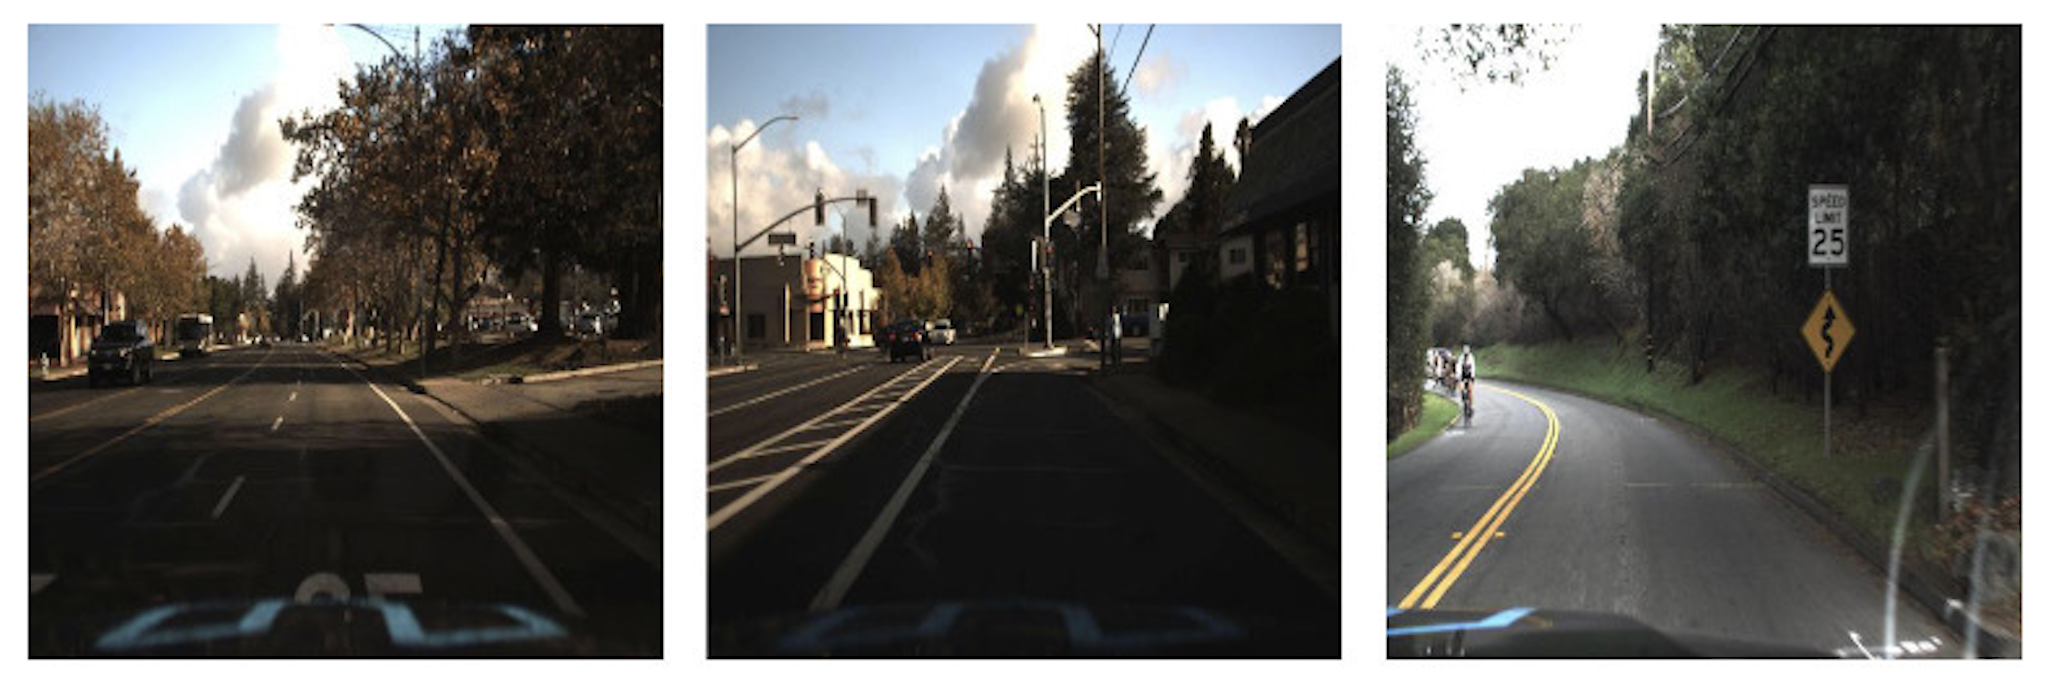
\includegraphics[width=0.55\linewidth]{datasetImages.png}
	\caption[Beispielbilder aus dem Datensatz]{Beispielbilder aus dem Datensatz. Quelle: \cite{datasetSelfDrivingCar}}
	\label{fig:datasetImages}
\end{figure}

Die Bilder in dem Datensatz umfassen verschiedene Szenarien im Straßenverkehr. Darunter befinden sich Stadt- und Landstraßen. Die Bilder wurden bei unterschiedlichen Lichtbedingungen aufgenommen, um ein breite Vielfalt an Situationen in den Daten abzudecken. 


\section{Klassenaufteilung}
Die ursprüngliche Klasseneinteilung ist in Abbildung \ref{fig:classDistributionRaw} dargestellt. Dort lässt sich erkennen, dass insbesondere die Aufteilung der Klasse \textit{Ampel} in Unterkategorien unterrepräsentiert ist. Um dieses Problem zu umgehen, wurden die \textit{Ampel}-Klassen zu einer Klasse \textit{trafficLight} zusammengeführt. Für das Auswerten des Datensatzes wurde dieser mit dem passenden Skript (datasetPreprocessing.ipynb) in einen Trainings-, Validierungs- und Testdatensatz aufgeteilt. Diese Aufteilung kann aus den farblichen Säulen in Abbildung \ref{fig:datasetTrainValTestSplit} entnommen werden. Eine weitere Bearbeitung des Datensatzes wurde nicht vorgenommen, um zu überprüfen, wie die verwendeten Netzwerke mit einem unbalancierten Datensatz umgehen. 

\begin{figure}
	\begin{subfigure}{0.5\textwidth}
		\centering
		\begin{tabular}{l|c|c}
			\hline
			Klassen & Anzahl & Index \\
			\hline
			\hline
			car & 64399 & 0 \\
			pedestrian & 10806 & 1 \\
			trafficLight-Red & 6870 & 2 \\
			trafficLight-Green & 5465 & 3 \\
			truck & 3623 & 4 \\
			trafficLight & 2568 & 5 \\
			biker & 1846 & 6 \\
			trafficLight-RedLeft & 1751 & 7 \\
			trafficLight-GreenLeft & 310 & 8 \\
			trafficLight-Yellow & 272 & 9 \\
			trafficLight-YellowLeft & 14 & 10 \\
			\hline
		\end{tabular}
		\caption{Klassenverteilung der rohen Daten als Tabelle. Quelle: Eigene Darstellung}
		\label{tab:classDistributionRaw_graph}
	\end{subfigure}%
	\begin{subfigure}{0.5\textwidth}
	\centering
	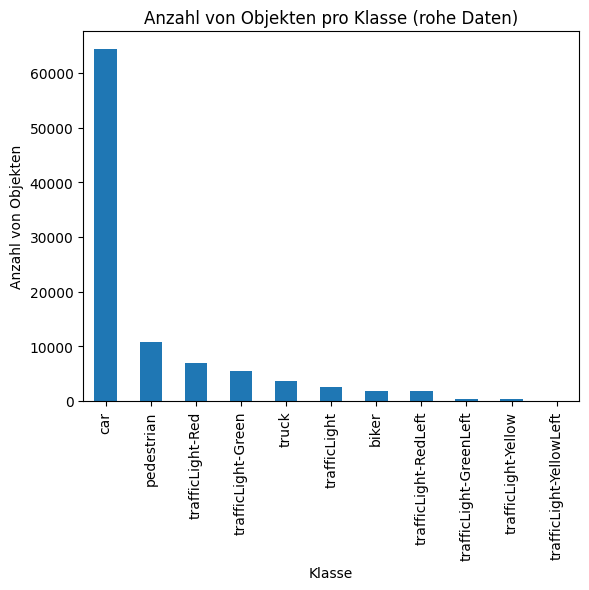
\includegraphics[width=\linewidth]{classDistribution_raw.png}
	\caption[Klassenverteilung der rohen Daten als Diagramm]{Klassenverteilung der rohen Daten als Diagramm. Quelle: Eigene Aufnahme}
	\label{fig:classDistributionRaw_graph}
	\end{subfigure}%
	\caption{Klassenverteilung der rohen Daten}
	\label{fig:classDistributionRaw}
\end{figure}


\begin{figure}
	\centering
		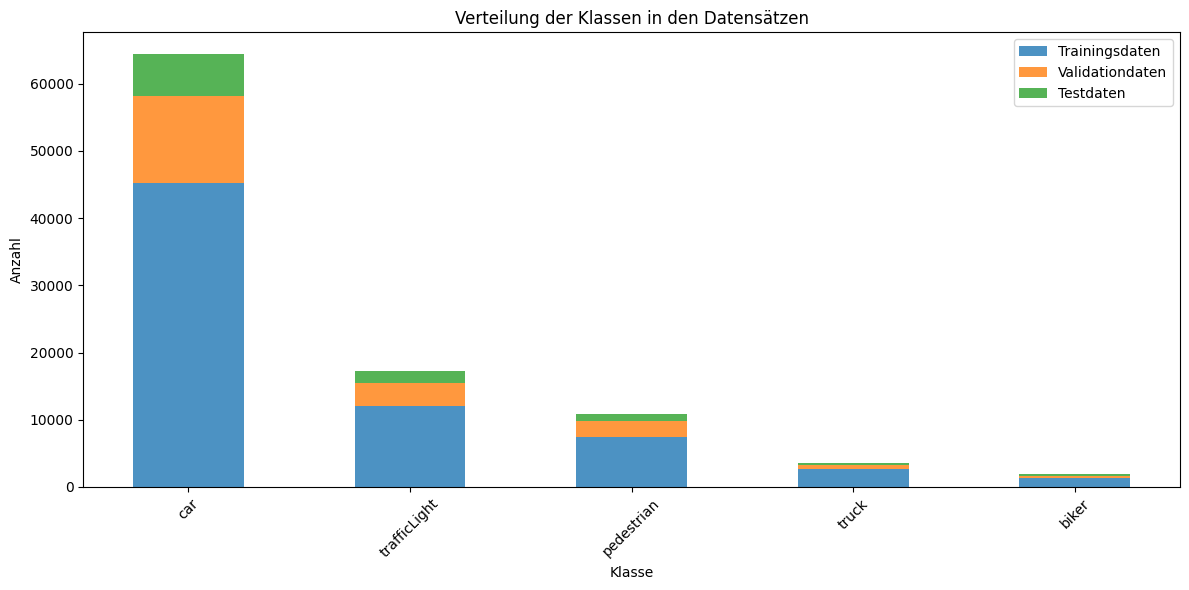
\includegraphics[width=\linewidth]{classDistribution_newClassesTrainValTest.png}
		\caption[Aufteilung in Trainings-, Validation- und Testdaten]{Aufteilung in Trainings-, Validation- und Testdaten. Quelle: Eigene Aufnahme}
		\label{fig:datasetTrainValTestSplit}
\end{figure}


\section{Aufbau}
\subsection{Rohdaten}
Die Rohdaten sind in einem Ordner gespeichert. Dieser Ordner enthält die Bilder im .jpg-Format und eine .csv-Datei in der alle Annotationen enthalten sind. Der Header der Datei enthält den Dateinamen des Bildes, die Breite und Höhe, die Klasse und die vier Bounding Box Koordinaten zu jedem Objekt.

Die folgenden Umwandlungen in die Formate werden mit dem Skript \textit{datasetConvertion.ipynb} gemacht. Die jeweiligen Ordnerstrukturen können in Kapitel \ref{chap:appendix} nachgelesen werden.


\subsection{YOLOX}
Das Netzwerk kann das COCO-Format und das PASCAL VOC-Format verarbeiten. In der folgenden Arbeit wird das COCO-Format verwendet. Zu diesem Zweck werden die Annotationen in einem separaten Ordner und die jeweiligen Bilddateien für Training, Validierung und Test, ebenfalls in einem separaten Ordner abgelegt. Die Annotationen zu den drei Teildatensätzen liegen im .json-Format vor. Dabei wird jeder Klasse, jedem Bild und jeder Annotation eine ID zugewiesen, die die Zuordnung der Objekte zu den jeweiligen Bildern ermöglicht. 



\subsection{YOLOv8}
Dieses Netzwerk verwendet das YOLO-Format. Dabei werden die Bilder für Training, Validierung und Test in einem separaten Ordner gespeichert. Die dazugehörigen Labels stehen in einzelnen .txt-Dateien. Jedes Bild erhält eine zugehörige Textdatei mit dem gleichen Namen wie das Bild und der Struktur Klasse, x-Zentrum, y-Zentrum, Breite und Höhe. Die Koordinaten müssen auf die Bildgröße normiert sein. Die Labels liegen in einer korrespondierenden Ordnerstruktur. Die zugehörige Konfigurationsdatei gibt anschließend den Pfad zu den Datensatz und die Anzahl der Klassen an. 



